\chapter{Evolution in multigene families}

We now know a lot about the dynamics of nucleotide substitutions
within existing genes, but we've neglected one key component of
molecular evolution. We haven't talked about where new genes come
from. It's important to understand this phenomenon because, after all,
new metabolic functions are likely to arise only when there are new
genes that can perform them. It's not likely that an existing gene can
adopt a new function while continuing to serve its old one.

Fundamentally the source of new genes is the {\it duplication\/} of
existing genes and their {\it divergence\/} in function. As we'll see
in a moment, for example, genes coding for myogblobin and hemoglobin
in mammals are descendants of a single common ancestor. That's the
duplication. Myoglobin is involved in oxygen metabolism in muscle,
while hemoglobin is involved in oxygen transport in blood. That's the
divergence. Although there are many interesting things to say about
the processes by which duplication and divergence occur, we're going
to focus on the pattern of nucleotide sequence evolution that arises
as a result.\index{duplication}\index{divergence}

\section*{Globin evolution}\index{globins}

I've just pointed out the distinction between myoglobin and
hemoglobin. You may also remember that hemoglobin is a multimeric
protein consisting of four subunits, 2 $\alpha$ subunits and 2 $\beta$
subunits. What you may not know is that in humans there are actually
two types of $\alpha$ hemoglobin and four types of $\beta$ hemoglobin,
each coded by a different genetic locus~(see
Table~\ref{table:globins}). The five $\alpha$-globin loci ($\alpha_1$,
$\alpha_2$, $\zeta$, and two non-functional pseudogenes) are found in a
cluster on chromosome 16. The six $\beta$-globin loci ($\epsilon$,
$\gamma_G$, $\gamma_A$, $\delta$, $\beta$, and a pseudogene) are found
in a cluster on chromosome 11. The myoglobin locus is on chromosome
22.

\begin{table}
\begin{center}
\begin{tabular}{l|cc}
\hline\hline
Developmental stage & $\alpha$ globin & $\beta$ globin \\
\hline
Embryo & $\zeta$  & $\epsilon$ \\
       & $\alpha$ & $\epsilon$ \\
Fetus  & $\alpha$ & $\beta$ \\
       & $\alpha$  & $\gamma$ \\
Adult  & $\alpha$ & $\beta$ \\
       & $\alpha$ & $\delta$ \\
\hline
\end{tabular}
\end{center}
\caption{Human hemoglobins arranged in developmental sequence. Adult
  hemoglobins composed of 2$\alpha$ and 2$\delta$ subunits typically
  account for less than 3\% of hemoglobins in adults (\myurl{http://sickle.bwh.harvard.edu/hbsynthesis.html}).}\label{table:globins}
\end{table}

Not only do we have all of these different types of globin genes in
our bodies, they're all related to one another. Comparative sequence
analysis has shown that vertebrate myoglobin and hemoglobins diverged
from one another about 450 million years ago. Figure~\ref{fig:globins}
shows a phylogenetic analysis of part of the globin gene family,
namely the $\beta$ globin genes within tetrapods. If you stare at this
tree for a while, you'll notice a couple of interesting things:

\begin{itemize}

\item Eutherian $\beta$ and $\delta$ globins are more closely related
  to marsupial $\beta$ globins than they are to eutherian $\epsilon$
  or $\gamma$ globins.

\item Marsupial $\beta$ globin is more closely related to eutherian
  $\beta$ and $\delta$ globins than it is to marsupial $\epsilon$
  globin. 

\end{itemize}

\begin{figure}
\begin{center}
\resizebox{0.9\textwidth}{!}{\includegraphics{globin-gene-tree.eps}}
\end{center}
\caption{Evolution of $\beta$-globin genes in tetrapods drawn as a
  gene tree~(from~\cite{Opazo-etal-2008}).}\label{fig:globins}
\end{figure}

\noindent To put that another way, $\beta$ globin genes within humans
(a eutherian) are more closely related to $\beta$ globin genes in
kangaroos (a marsupial) than to $\epsilon$ globin genes in
humans. Strange as it seems, this pattern is exactly what we expect as
a result of duplication and divergence. 

Up to the time that a gene becomes duplicated, its evolutionary
history matches the evolutionary history of the organisms containing
it.  Once there are duplicate copies, each follows an independent
evolutionary history. Each traces the history of speciation and
divergence. And over long periods duplicate copies of the same gene
share more recent common ancestry with copies of the same gene in a
different species than they do with duplicate genes in the same
genome. You can see that in this example if we redraw the gene tree in
Figure~ref{fig:globins} as a species tree with the gene tree inside
it~(Figure~\ref{fig:globins-species}). 

\begin{figure}
\begin{center}
\resizebox{0.9\textwidth}{!}{\includegraphics{globin-species-tree.eps}}
\end{center}
\caption{Evolution of $\beta$-globin genes in tetrapods drawn as a
  species tree~(from~\cite{Opazo-etal-2008}).}\label{fig:globins-species}
\end{figure}

A history of duplication and divergence in multigene families makes it
important to distinguish between two classes of related loci: those
that represent the same locus in different species and between which
divergence is a result of species divergence are {\it
  orthologs}.\index{orthology}\index{multigene family!ortholog} Those
that represent different loci and between which divergence occurred
after duplication of an ancestral gene are {\it
  paralogs}.\index{paralogy}\index{multigene family!paralog} The
$\beta$-globin loci of humans and chickens are orthologous. The
$\alpha$- and $\beta$-globin loci of any pair of taxa are paralogous.

As multigene families go, the globin family is relatively simple and
easy to understand. There are only about a dozen loci involved, one
isolated locus (myoglobin) and two clusters of loci ($\alpha$- and
$\beta$-globins). You'll find a diagram of the $\beta$-globin cluster
in Figure~\ref{fig:beta-globin}. As you can see the $\beta$-globins
are not only evolutionarily related to one another they occur
relatively close to one another on chromosome 11 in humans.

\begin{figure}
\begin{center}
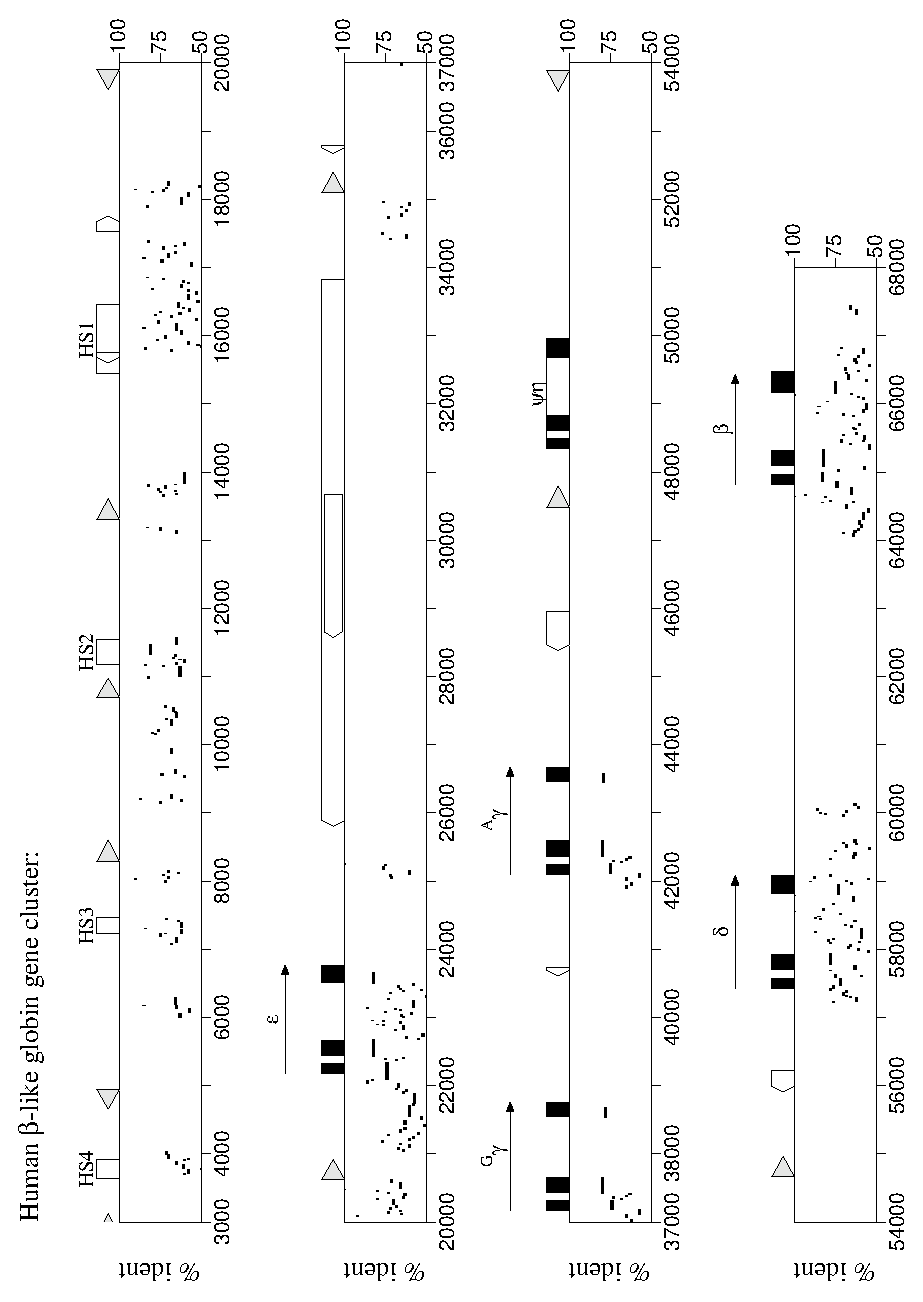
\includegraphics[angle=270,scale=0.5]{beta-globin.eps}
\caption{Structure of the human $\beta$-globin gene cluster. \%
  identity refers to similarity to the mouse $\beta$-globin
  sequence. From
  \myurl{http://globin.cse.psu.edu/html/pip/betaglobin/iplot.ps}
  (retrieved 28 Nov 2006).}\label{fig:beta-globin}
\end{center}
\end{figure}

Other families are far more complex. Class I and class II MHC loci,
for example are part of the same multigene family. Moreover,
immunoglobulins, T-cell receptors, and, and MHC loci are part of a
larger superfamily of genes, i.e., all are ultimately derived from a
common ancestral gene by duplication and
divergence. Table~\ref{table:superfamilies} lists a few examples of
multigene families and superfamilies in the human genome and the
number of proteins produced.\index{multigene family!examples}

\begin{table}
\begin{center}
\begin{tabular}{ll}
\hline\hline
Protein family domain & Number of proteins \\
\hline
Actin                 & 61 \\
Immunoglobulin        & 381 \\
Fibronectin type I    & 5 \\
Fibronectin type II   & 11 \\
Fibronectin type III  & 106 \\
Histone \\
\quad H2A/H2B/H3/H4   & 75 \\
Homeobox              & 160 \\
Immunoglobulin        & 381 \\
MHC Class I           & 18 \\
MHC Class II$\alpha$  & 5 \\
MHC Class II$\beta$   & 7 \\
T-cell receptor $\alpha$ & 16 \\
T-cell receptor $\beta$  & 15 \\
T-cell receptor $\gamma$ & 1 \\
T-cell receptor $\delta$ & 1 \\
Zinc finger, C2H2     & 564 \\
Zinc finger, C3HC4    & 135 \\
\hline
\end{tabular}
\end{center}
\caption{A few gene families from the human genome~(adapted from~\cite{Ohta2003,Venter-etal2001}).}\label{table:superfamilies}
\end{table}

\section*{Concerted evolution}\index{concerted evolution}
\index{multigene family!concerted evolution}

Although the patterns of gene relationships produced through
duplication and divergence can be quite complex, the processes are
relatively easy to understand. In some multigene families, however,
something quite different seems to be going on. In many plants and
animals, genes encoding ribosomal RNAs are present in hundreds of
copies and arranged end to end in long tandem arrays in one or a few
places in the genome~(Figure~\ref{fig:rdna}). Brown et
al.~\cite{Brown-etal72} compared the ribosomal RNA of {\it Xenopus
  laevis\/} and {\it X. mulleri\/} and found a surprising
pattern. There was little or no detectable variation among copies of
the repeat units within either species, in spite of substantial
divergence between them. This pattern can't be explained by purifying
selection. Members of the gene family presumably diverged before {\it
  X. laevis\/} and {\it X. mulleri\/} diverged. Thus, we would expect
more divergence among copies {\it within\/} species than {\it
  between\/} species, i.e., the pattern we see in the globin
family. Explaining this pattern requires some mechanism that causes
different copies of the repeat to be homogenized within each species
while allowing the repeats to diverge between species. The phenomenon
is referred to as concerted evolution.

\begin{figure}
\begin{center}
\resizebox{0.75\textwidth}{!}{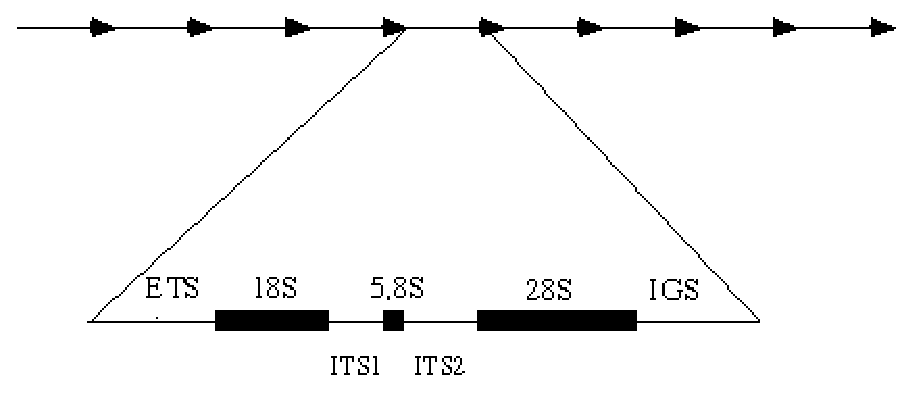
\includegraphics{rdna.eps}}
\end{center}
\caption{Diagrammatic representation of ribosomal DNA in vascular
  plant genomes~(from Muir \& Schl{\"o}tterer, 1999
  \myurl{http://webdoc.sub.gwdg.de/ebook/y/1999/whichmarker/m11/Chap11.htm}).}\label{fig:rdna}
\end{figure}

Two mechanisms that can result in concerted evolution have been widely
studied: unequal crossing over and gene conversion.  \index{multigene family!unequal crossing over} \index{multigene family!gene conversion} \index{unequal crossing over} \index{gene conversion}
Both depend on misalignments during meiotic prophase. These
misalignments allow a mutation that occurs in one copy of a tandemly
repeated gene array to ``spread'' to other copies of the gene
array. Tomoko Ohta and Thomas Nagylaki have provided exhaustive
mathematical treatments of the process~\cite{Nagylaki84,Ohta84}. We'll
follow Ohta's treatment, but keep it fairly simple and
straightforward. First some notation:\footnote{See
Figure~\ref{fig:ohta-multigene} for a diagram that you may find
helpful}
\begin{eqnarray*}
f   &=& \mbox{P}(\mbox{two alleles at same locus are ibd}) \\
c_1 &=& \mbox{P}(\mbox{two alleles at different loci in same
  chromosome are ibd}) \\
c_2 &=& \mbox{P}(\mbox{two alleles at different loci in different
  chromosomes are ibd}) \\
\mu &=& \mbox{mutation rate} \\
n &=& \mbox{no.\ of loci in family} \\
\lambda &=& \mbox{rate of gene conversion}
\end{eqnarray*}

\begin{figure}
\resizebox{\textwidth}{!}{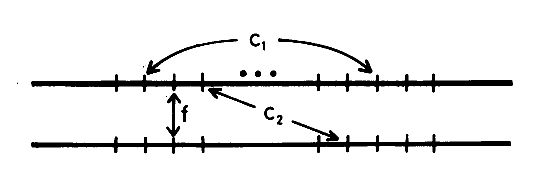
\includegraphics{ohta-multigene.eps}}
\caption{Types of identity by descent within a tandem
  repeat~(from~\cite{Ohta-1982}).}\label{fig:ohta-multigene}
\end{figure}

Now remember that for the infinite alleles model
\[
f = \frac{1}{4N_e\mu + 1} \quad , \\
\]
and $f$ is the probability that neither allele has undergone
mutation. By analogy
\[
g = \frac{1}{4N_e\lambda + 1} \quad , \\
\]
where $g$ is the probability that two alleles at a homologous position
are ibd in the sense that neither has ever moved from that position in
the array. Thus, for our model
\begin{eqnarray*}
f &=& P(\mbox{neither has moved})\mbox{P}(\mbox{ibd}) \\
  && + \mbox{P}(\mbox{one has moved})\mbox{P}(\mbox{ibd anyway}) \\
  &=&
  \left(\frac{1}{4N_e\lambda+1}\right)\left(\frac{1}{4N_e\mu+1}\right) 
  + \left(\frac{4N_e\lambda}{4N_e\lambda+1}\right)c_2 \\
  &\approx& \frac{4N_e\lambda c_2 + 1}{4N_e\lambda + 4N_e\mu + 1}
  \\
c_1 = c_2 &=& \frac{\lambda}{\lambda + (n-1)\mu} \quad .
\end{eqnarray*}

Notice that $(n-1)\mu$ is approximately the number of mutations that
occur in a single array every generation. Consider two possibilities:

\begin{itemize}

\item {\it Gene conversion occurs much more often than mutation\/}:
  $\lambda \gg (n-1)\mu$.

Under these conditions $c_2 \approx 1$ and $f \approx 1$. In short,
all copies of alleles at every locus in the array are virtually
identical{\dash}concerted evolution.

\item {\it Gene conversion occurs much less often than mutation\/}:
  $\lambda \ll (n-1)\mu$.

Under these conditions $c_2 \approx 0$ and $f \approx \frac{1}{4N_e\mu
  + 1}$. In short, copies of alleles at different loci are almost
  certain to be different from one another, and the diversity at any
  single locus matches neutral expectations{\dash}non-concerted
  evolution.

\end{itemize}

